\section{Basics of Reinforcement Learning}
\label{sec:reinforcement_learning}

\begin{frame}{Markov Decision Processes}
	\begin{block}{Reinforcement Learning}
		General class of algorithms that allow an agent to learn how to behave
		in a stochastic and possibly unknown environment by trial-and-error.
	\end{block}
	
	\begin{block}{Markov Decision Process (MDP)}
		stochastic dynamical system specified by $<\S, \A, \calP, \calR, \gamma>$
		\begin{enumerate}
			\item $(\S, \calS)$ is a measurable state space
			\item $(\A, \calA)$ is a measurable action space
			\item $\calP: \S \times \A \times \calS \to \R$ is a Markov transition kernel
			\item $\calR: \S \times \A \to \R$ is a reward function
			\item $0 < \gamma < 1$ is the discount factor.
		\end{enumerate}
	\end{block}
\end{frame}

\begin{frame}{Interaction Between Agent and Environment}
\begin{figure}[t]
	\centering
	\begin{tikzpicture}[node distance = 6em, auto, thick]
		\node [block] (Agent) {Agent\\$\pi$};
		\node [block, below of=Agent] (Environment) {Environment\\$\calP, \calR$};		    
		\path [line] (Agent.0) --++ (4em,0em) |- node [near start]{Action $a_t$} (Environment.0);
		\path [line] (Environment.190) --++ (-6em,0em) |- node [near start]{State  $s_{t}$} (Agent.170);
		\path [line] (Environment.170) --++ (-4.25em,0em) |- node [near start, right] {Reward $r_{t+1}$} (Agent.190);
	\end{tikzpicture}
\end{figure}
\end{frame}

\begin{frame}{Policy and Value Function}
	\begin{block}{Policy}
		 A policy is a function $\pi: \S \times \A \to \R$ such that, $\forall s \in \S$, $C \mapsto \pi(s,C)$ is a probability distribution over $(\A, \calA)$
	\end{block}
	\begin{block}{Return}
		\begin{equation*}
			G_t = \sum^{\infty}_{t=0} \gamma^t R_{t+k+1} 
		\end{equation*}
	\end{block}
	\begin{block}{Value Function}
		\begin{equation*}
			V_\pi(s) = \E[\pi]{G_t|S_t = s}
		\end{equation*}
	\end{block}
	\begin{block}{Agent's goal}
		Select a policy $\pi^*$ that maximizes his expected return in all possible states. This policy is called \emph{optimal}.
	\end{block}
\end{frame}

\begin{frame}{Policy Gradient Methods}
	\begin{block}{Key idea}
	$\pi_*$ is approximated using a parametrized policy $\pi_{\theta^*}(s,a)$, where
	\begin{equation*}
		\theta^* = \argmax_{\theta \in \Theta} J(\theta) = V_{\pi_\theta}(s_0)
	\end{equation*}
	Using gradient descent, we have the following update scheme
	\begin{equation*}
		\theta_{k+1} = \theta_k + \alpha_k \nabla_\theta J\left(\theta_k\right)
	\end{equation*}
	\end{block}

	\begin{block}{Policy Gradient Theorem}
			Let $\pi_\theta$ be a differentiable policy. The policy gradient for the average reward formulation is given by
			\begin{equation*}
				\nabla_\theta J(\theta) =
				\E[\substack{S \sim d^\theta\\A \sim \pi_\theta}]{\nabla_\theta\log
				\pi_\theta(S,A) Q_{\theta}(S, A)}
			\end{equation*}
			$d^\theta$ is the stationary distribution of the Markov chain induced by $\pi_\theta$.
	\end{block}
\end{frame}

\begin{frame}{Monte-Carlo Policy Gradient Method}
	\begin{figure}[h]
		\centering
		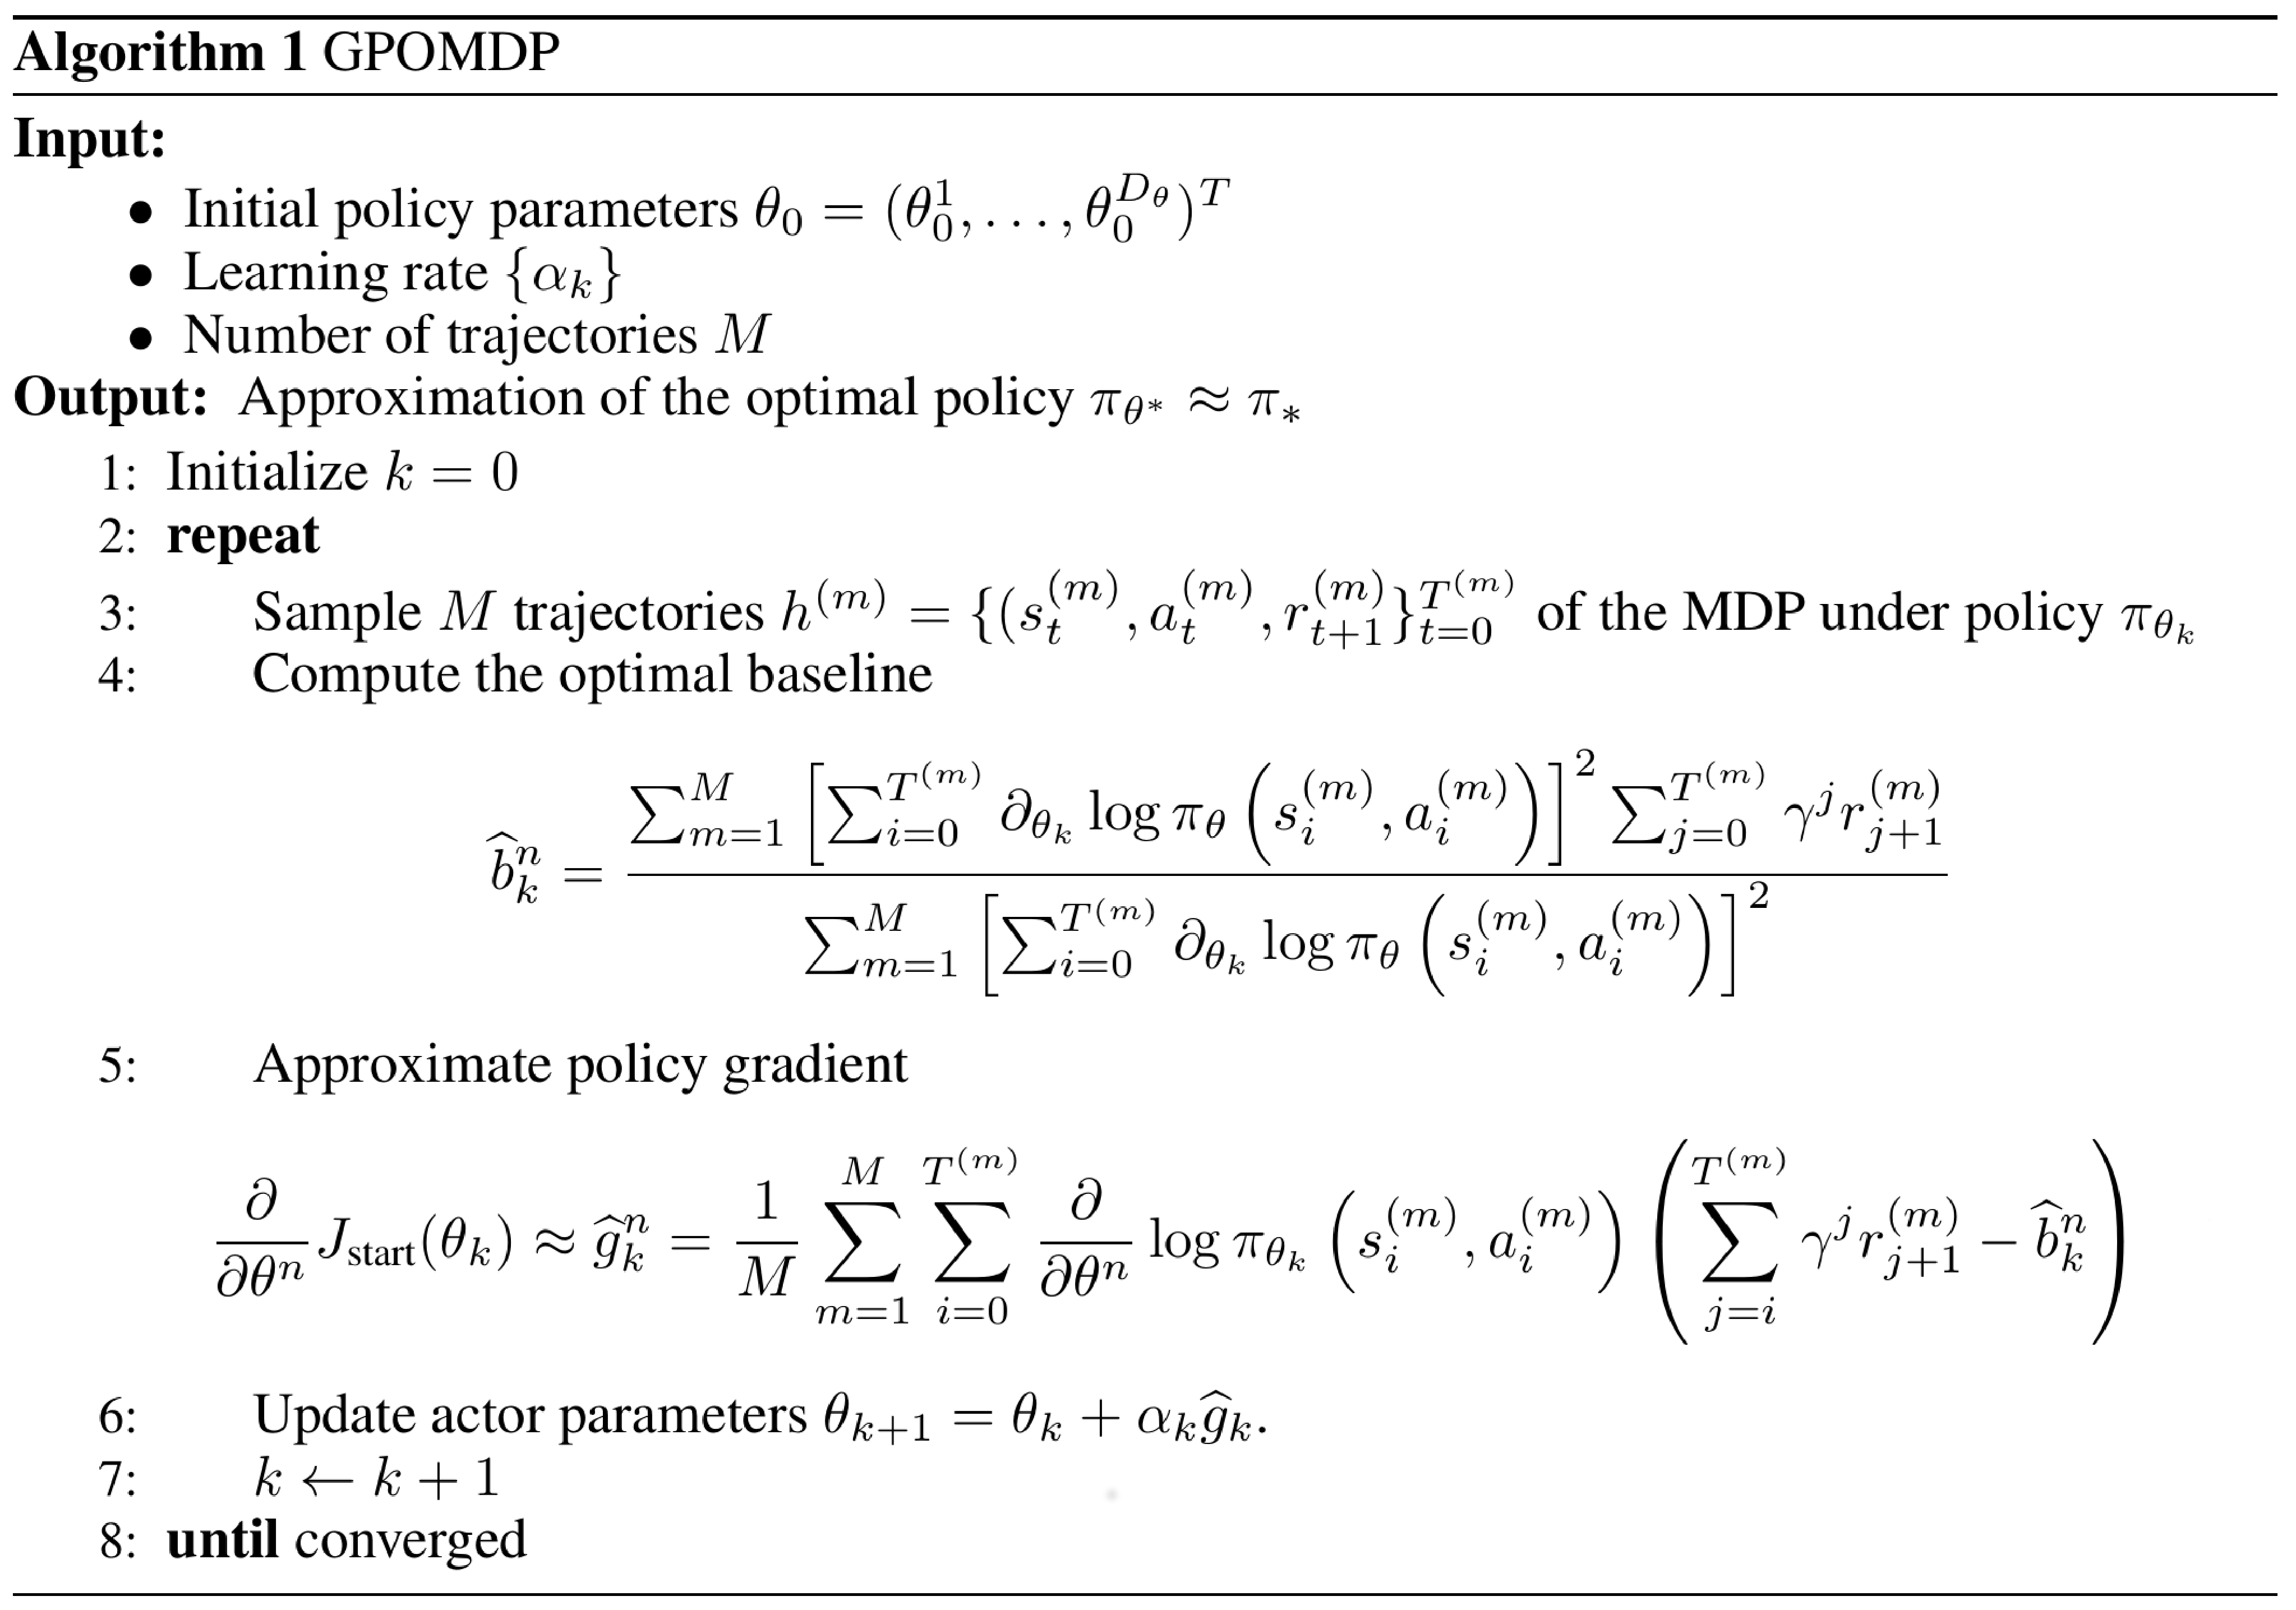
\includegraphics[width=1.0\framewidth]{Images/gpomdp}
	\end{figure}
\end{frame}
